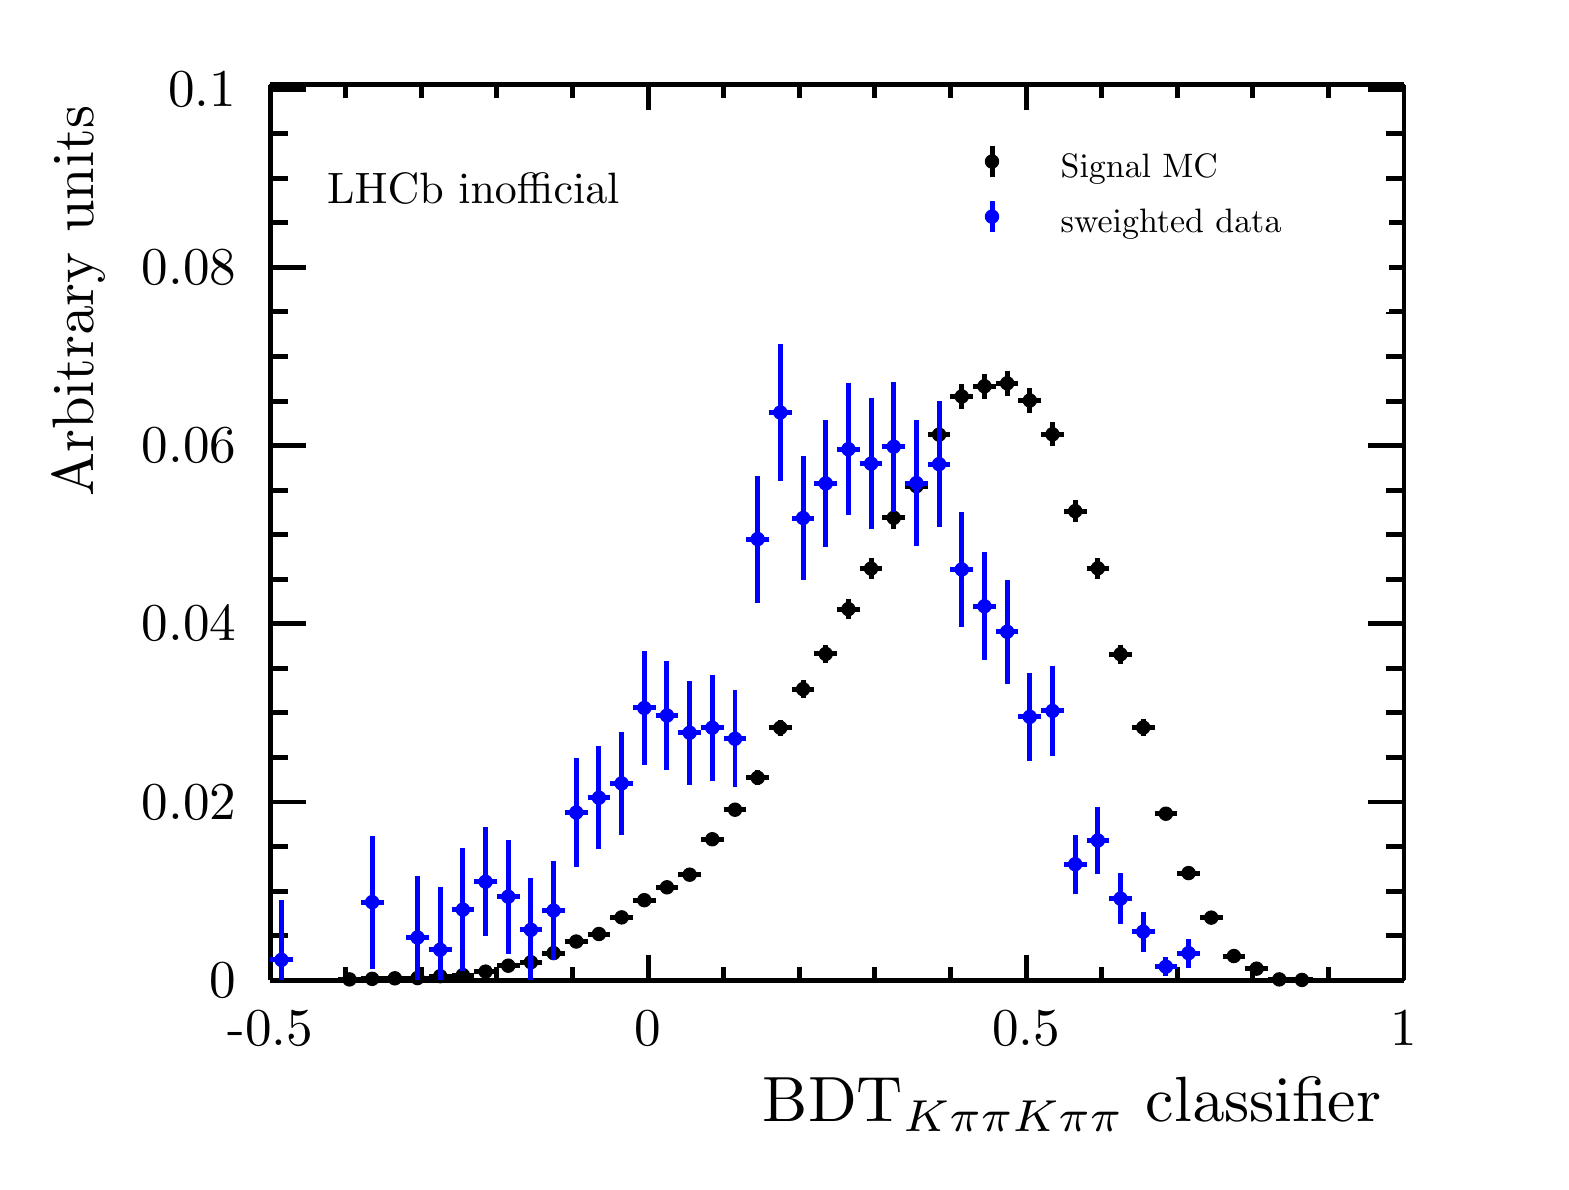
\begin{tikzpicture}
\pgfdeclareplotmark{cross} {
\pgfpathmoveto{\pgfpoint{-0.3\pgfplotmarksize}{\pgfplotmarksize}}
\pgfpathlineto{\pgfpoint{+0.3\pgfplotmarksize}{\pgfplotmarksize}}
\pgfpathlineto{\pgfpoint{+0.3\pgfplotmarksize}{0.3\pgfplotmarksize}}
\pgfpathlineto{\pgfpoint{+1\pgfplotmarksize}{0.3\pgfplotmarksize}}
\pgfpathlineto{\pgfpoint{+1\pgfplotmarksize}{-0.3\pgfplotmarksize}}
\pgfpathlineto{\pgfpoint{+0.3\pgfplotmarksize}{-0.3\pgfplotmarksize}}
\pgfpathlineto{\pgfpoint{+0.3\pgfplotmarksize}{-1.\pgfplotmarksize}}
\pgfpathlineto{\pgfpoint{-0.3\pgfplotmarksize}{-1.\pgfplotmarksize}}
\pgfpathlineto{\pgfpoint{-0.3\pgfplotmarksize}{-0.3\pgfplotmarksize}}
\pgfpathlineto{\pgfpoint{-1.\pgfplotmarksize}{-0.3\pgfplotmarksize}}
\pgfpathlineto{\pgfpoint{-1.\pgfplotmarksize}{0.3\pgfplotmarksize}}
\pgfpathlineto{\pgfpoint{-0.3\pgfplotmarksize}{0.3\pgfplotmarksize}}
\pgfpathclose
\pgfusepathqstroke
}
\pgfdeclareplotmark{cross*} {
\pgfpathmoveto{\pgfpoint{-0.3\pgfplotmarksize}{\pgfplotmarksize}}
\pgfpathlineto{\pgfpoint{+0.3\pgfplotmarksize}{\pgfplotmarksize}}
\pgfpathlineto{\pgfpoint{+0.3\pgfplotmarksize}{0.3\pgfplotmarksize}}
\pgfpathlineto{\pgfpoint{+1\pgfplotmarksize}{0.3\pgfplotmarksize}}
\pgfpathlineto{\pgfpoint{+1\pgfplotmarksize}{-0.3\pgfplotmarksize}}
\pgfpathlineto{\pgfpoint{+0.3\pgfplotmarksize}{-0.3\pgfplotmarksize}}
\pgfpathlineto{\pgfpoint{+0.3\pgfplotmarksize}{-1.\pgfplotmarksize}}
\pgfpathlineto{\pgfpoint{-0.3\pgfplotmarksize}{-1.\pgfplotmarksize}}
\pgfpathlineto{\pgfpoint{-0.3\pgfplotmarksize}{-0.3\pgfplotmarksize}}
\pgfpathlineto{\pgfpoint{-1.\pgfplotmarksize}{-0.3\pgfplotmarksize}}
\pgfpathlineto{\pgfpoint{-1.\pgfplotmarksize}{0.3\pgfplotmarksize}}
\pgfpathlineto{\pgfpoint{-0.3\pgfplotmarksize}{0.3\pgfplotmarksize}}
\pgfpathclose
\pgfusepathqfillstroke
}
\pgfdeclareplotmark{newstar} {
\pgfpathmoveto{\pgfqpoint{0pt}{\pgfplotmarksize}}
\pgfpathlineto{\pgfqpointpolar{44}{0.5\pgfplotmarksize}}
\pgfpathlineto{\pgfqpointpolar{18}{\pgfplotmarksize}}
\pgfpathlineto{\pgfqpointpolar{-20}{0.5\pgfplotmarksize}}
\pgfpathlineto{\pgfqpointpolar{-54}{\pgfplotmarksize}}
\pgfpathlineto{\pgfqpointpolar{-90}{0.5\pgfplotmarksize}}
\pgfpathlineto{\pgfqpointpolar{234}{\pgfplotmarksize}}
\pgfpathlineto{\pgfqpointpolar{198}{0.5\pgfplotmarksize}}
\pgfpathlineto{\pgfqpointpolar{162}{\pgfplotmarksize}}
\pgfpathlineto{\pgfqpointpolar{134}{0.5\pgfplotmarksize}}
\pgfpathclose
\pgfusepathqstroke
}
\pgfdeclareplotmark{newstar*} {
\pgfpathmoveto{\pgfqpoint{0pt}{\pgfplotmarksize}}
\pgfpathlineto{\pgfqpointpolar{44}{0.5\pgfplotmarksize}}
\pgfpathlineto{\pgfqpointpolar{18}{\pgfplotmarksize}}
\pgfpathlineto{\pgfqpointpolar{-20}{0.5\pgfplotmarksize}}
\pgfpathlineto{\pgfqpointpolar{-54}{\pgfplotmarksize}}
\pgfpathlineto{\pgfqpointpolar{-90}{0.5\pgfplotmarksize}}
\pgfpathlineto{\pgfqpointpolar{234}{\pgfplotmarksize}}
\pgfpathlineto{\pgfqpointpolar{198}{0.5\pgfplotmarksize}}
\pgfpathlineto{\pgfqpointpolar{162}{\pgfplotmarksize}}
\pgfpathlineto{\pgfqpointpolar{134}{0.5\pgfplotmarksize}}
\pgfpathclose
\pgfusepathqfillstroke
}
\definecolor{c}{rgb}{1,1,1};
\draw [color=c, fill=c] (0.4,0) rectangle (19.6,14.393);
\draw [color=c, fill=c] (3.472,2.30288) rectangle (17.872,13.6733);
\definecolor{c}{rgb}{0,0,0};
\draw [c,line width=0.9] (3.472,2.30288) -- (3.472,13.6733) -- (17.872,13.6733) -- (17.872,2.30288) -- (3.472,2.30288);
\definecolor{c}{rgb}{1,1,1};
\draw [color=c, fill=c] (3.472,2.30288) rectangle (17.872,13.6733);
\definecolor{c}{rgb}{0,0,0};
\draw [c,line width=0.9] (3.472,2.30288) -- (3.472,13.6733) -- (17.872,13.6733) -- (17.872,2.30288) -- (3.472,2.30288);
\draw [c,line width=1.8] (4.336,2.31311) -- (4.42987,2.31311);
\draw [c,line width=1.8] (4.53013,2.31311) -- (4.624,2.31311);
\foreach \P in {(4.48,2.31311)}{\draw[mark options={color=c,fill=c},mark size=2.402402pt,mark=*] plot coordinates {\P};}
\draw [c,line width=1.8] (4.624,2.31993) -- (4.71787,2.31993);
\draw [c,line width=1.8] (4.81813,2.31993) -- (4.912,2.31993);
\foreach \P in {(4.768,2.31993)}{\draw[mark options={color=c,fill=c},mark size=2.402402pt,mark=*] plot coordinates {\P};}
\draw [c,line width=1.8] (4.912,2.32675) -- (5.00587,2.32675);
\draw [c,line width=1.8] (5.10613,2.32675) -- (5.2,2.32675);
\foreach \P in {(5.056,2.32675)}{\draw[mark options={color=c,fill=c},mark size=2.402402pt,mark=*] plot coordinates {\P};}
\draw [c,line width=1.8] (5.2,2.33016) -- (5.29387,2.33016);
\draw [c,line width=1.8] (5.39413,2.33016) -- (5.488,2.33016);
\foreach \P in {(5.344,2.33016)}{\draw[mark options={color=c,fill=c},mark size=2.402402pt,mark=*] plot coordinates {\P};}
\draw [c,line width=1.8] (5.488,2.35403) -- (5.58187,2.35403);
\draw [c,line width=1.8] (5.68213,2.35403) -- (5.776,2.35403);
\foreach \P in {(5.632,2.35403)}{\draw[mark options={color=c,fill=c},mark size=2.402402pt,mark=*] plot coordinates {\P};}
\draw [c,line width=1.8] (5.776,2.36767) -- (5.86987,2.36767);
\draw [c,line width=1.8] (5.97013,2.36767) -- (6.064,2.36767);
\foreach \P in {(5.92,2.36767)}{\draw[mark options={color=c,fill=c},mark size=2.402402pt,mark=*] plot coordinates {\P};}
\draw [c,line width=1.8] (6.064,2.412) -- (6.15787,2.412);
\draw [c,line width=1.8] (6.25813,2.412) -- (6.352,2.412);
\foreach \P in {(6.208,2.412)}{\draw[mark options={color=c,fill=c},mark size=2.402402pt,mark=*] plot coordinates {\P};}
\draw [c,line width=1.8] (6.352,2.48701) -- (6.44587,2.48701);
\draw [c,line width=1.8] (6.54613,2.48701) -- (6.64,2.48701);
\foreach \P in {(6.496,2.48701)}{\draw[mark options={color=c,fill=c},mark size=2.402402pt,mark=*] plot coordinates {\P};}
\draw [c,line width=1.8] (6.64,2.53134) -- (6.73387,2.53134);
\draw [c,line width=1.8] (6.83413,2.53134) -- (6.928,2.53134);
\foreach \P in {(6.784,2.53134)}{\draw[mark options={color=c,fill=c},mark size=2.402402pt,mark=*] plot coordinates {\P};}
\draw [c,line width=1.8] (6.928,2.64728) -- (7.02187,2.64728);
\draw [c,line width=1.8] (7.12213,2.64728) -- (7.216,2.64728);
\foreach \P in {(7.072,2.64728)}{\draw[mark options={color=c,fill=c},mark size=2.402402pt,mark=*] plot coordinates {\P};}
\draw [c,line width=1.8] (7.216,2.79391) -- (7.30987,2.79391);
\draw [c,line width=1.8] (7.41013,2.79391) -- (7.504,2.79391);
\foreach \P in {(7.36,2.79391)}{\draw[mark options={color=c,fill=c},mark size=2.402402pt,mark=*] plot coordinates {\P};}
\draw [c,line width=1.8] (7.504,2.88939) -- (7.59787,2.88939);
\draw [c,line width=1.8] (7.69813,2.88939) -- (7.792,2.88939);
\foreach \P in {(7.648,2.88939)}{\draw[mark options={color=c,fill=c},mark size=2.402402pt,mark=*] plot coordinates {\P};}
\draw [c,line width=1.8] (7.936,3.04864) -- (7.936,3.05068);
\draw [c,line width=1.8] (7.936,3.15093) -- (7.936,3.15297);
\draw [c,line width=1.8] (7.792,3.1008) -- (7.88587,3.1008);
\draw [c,line width=1.8] (7.98613,3.1008) -- (8.08,3.1008);
\foreach \P in {(7.936,3.1008)}{\draw[mark options={color=c,fill=c},mark size=2.402402pt,mark=*] plot coordinates {\P};}
\draw [c,line width=1.8] (8.224,3.26018) -- (8.224,3.26891);
\draw [c,line width=1.8] (8.224,3.36917) -- (8.224,3.37791);
\draw [c,line width=1.8] (8.08,3.31904) -- (8.17387,3.31904);
\draw [c,line width=1.8] (8.27413,3.31904) -- (8.368,3.31904);
\foreach \P in {(8.224,3.31904)}{\draw[mark options={color=c,fill=c},mark size=2.402402pt,mark=*] plot coordinates {\P};}
\draw [c,line width=1.8] (8.512,3.41929) -- (8.512,3.43259);
\draw [c,line width=1.8] (8.512,3.53284) -- (8.512,3.54615);
\draw [c,line width=1.8] (8.368,3.48272) -- (8.46187,3.48272);
\draw [c,line width=1.8] (8.56213,3.48272) -- (8.656,3.48272);
\foreach \P in {(8.512,3.48272)}{\draw[mark options={color=c,fill=c},mark size=2.402402pt,mark=*] plot coordinates {\P};}
\draw [c,line width=1.8] (8.8,3.57539) -- (8.8,3.59286);
\draw [c,line width=1.8] (8.8,3.69311) -- (8.8,3.71058);
\draw [c,line width=1.8] (8.656,3.64298) -- (8.74988,3.64298);
\draw [c,line width=1.8] (8.85013,3.64298) -- (8.944,3.64298);
\foreach \P in {(8.8,3.64298)}{\draw[mark options={color=c,fill=c},mark size=2.402402pt,mark=*] plot coordinates {\P};}
\draw [c,line width=1.8] (9.088,4.01497) -- (9.088,4.04297);
\draw [c,line width=1.8] (9.088,4.14322) -- (9.088,4.17123);
\draw [c,line width=1.8] (8.944,4.0931) -- (9.03787,4.0931);
\draw [c,line width=1.8] (9.13813,4.0931) -- (9.232,4.0931);
\foreach \P in {(9.088,4.0931)}{\draw[mark options={color=c,fill=c},mark size=2.402402pt,mark=*] plot coordinates {\P};}
\draw [c,line width=1.8] (9.376,4.38226) -- (9.376,4.41807);
\draw [c,line width=1.8] (9.376,4.51832) -- (9.376,4.55412);
\draw [c,line width=1.8] (9.232,4.46819) -- (9.32587,4.46819);
\draw [c,line width=1.8] (9.42613,4.46819) -- (9.52,4.46819);
\foreach \P in {(9.376,4.46819)}{\draw[mark options={color=c,fill=c},mark size=2.402402pt,mark=*] plot coordinates {\P};}
\draw [c,line width=1.8] (9.664,4.78034) -- (9.664,4.82385);
\draw [c,line width=1.8] (9.664,4.9241) -- (9.664,4.96761);
\draw [c,line width=1.8] (9.52,4.87397) -- (9.61387,4.87397);
\draw [c,line width=1.8] (9.71413,4.87397) -- (9.808,4.87397);
\foreach \P in {(9.664,4.87397)}{\draw[mark options={color=c,fill=c},mark size=2.402402pt,mark=*] plot coordinates {\P};}
\draw [c,line width=1.8] (9.952,5.40368) -- (9.952,5.4581);
\draw [c,line width=1.8] (9.952,5.55835) -- (9.952,5.61277);
\draw [c,line width=1.8] (9.808,5.50822) -- (9.90187,5.50822);
\draw [c,line width=1.8] (10.0021,5.50822) -- (10.096,5.50822);
\foreach \P in {(9.952,5.50822)}{\draw[mark options={color=c,fill=c},mark size=2.402402pt,mark=*] plot coordinates {\P};}
\draw [c,line width=1.8] (10.24,5.88699) -- (10.24,5.94913);
\draw [c,line width=1.8] (10.24,6.04938) -- (10.24,6.11153);
\draw [c,line width=1.8] (10.096,5.99926) -- (10.1899,5.99926);
\draw [c,line width=1.8] (10.2901,5.99926) -- (10.384,5.99926);
\foreach \P in {(10.24,5.99926)}{\draw[mark options={color=c,fill=c},mark size=2.402402pt,mark=*] plot coordinates {\P};}
\draw [c,line width=1.8] (10.528,6.3271) -- (10.528,6.39583);
\draw [c,line width=1.8] (10.528,6.49608) -- (10.528,6.56482);
\draw [c,line width=1.8] (10.384,6.44596) -- (10.4779,6.44596);
\draw [c,line width=1.8] (10.5781,6.44596) -- (10.672,6.44596);
\foreach \P in {(10.528,6.44596)}{\draw[mark options={color=c,fill=c},mark size=2.402402pt,mark=*] plot coordinates {\P};}
\draw [c,line width=1.8] (10.816,6.88865) -- (10.816,6.96529);
\draw [c,line width=1.8] (10.816,7.06554) -- (10.816,7.14218);
\draw [c,line width=1.8] (10.672,7.01542) -- (10.7659,7.01542);
\draw [c,line width=1.8] (10.8661,7.01542) -- (10.96,7.01542);
\foreach \P in {(10.816,7.01542)}{\draw[mark options={color=c,fill=c},mark size=2.402402pt,mark=*] plot coordinates {\P};}
\draw [c,line width=1.8] (11.104,7.39681) -- (11.104,7.4802);
\draw [c,line width=1.8] (11.104,7.58045) -- (11.104,7.66383);
\draw [c,line width=1.8] (10.96,7.53032) -- (11.0539,7.53032);
\draw [c,line width=1.8] (11.1541,7.53032) -- (11.248,7.53032);
\foreach \P in {(11.104,7.53032)}{\draw[mark options={color=c,fill=c},mark size=2.402402pt,mark=*] plot coordinates {\P};}
\draw [c,line width=1.8] (11.392,8.0333) -- (11.392,8.12467);
\draw [c,line width=1.8] (11.392,8.22493) -- (11.392,8.3163);
\draw [c,line width=1.8] (11.248,8.1748) -- (11.3419,8.1748);
\draw [c,line width=1.8] (11.4421,8.1748) -- (11.536,8.1748);
\foreach \P in {(11.392,8.1748)}{\draw[mark options={color=c,fill=c},mark size=2.402402pt,mark=*] plot coordinates {\P};}
\draw [c,line width=1.8] (11.68,8.4309) -- (11.68,8.52705);
\draw [c,line width=1.8] (11.68,8.6273) -- (11.68,8.72344);
\draw [c,line width=1.8] (11.536,8.57717) -- (11.6299,8.57717);
\draw [c,line width=1.8] (11.7301,8.57717) -- (11.824,8.57717);
\foreach \P in {(11.68,8.57717)}{\draw[mark options={color=c,fill=c},mark size=2.402402pt,mark=*] plot coordinates {\P};}
\draw [c,line width=1.8] (11.968,9.07817) -- (11.968,9.18176);
\draw [c,line width=1.8] (11.968,9.28201) -- (11.968,9.38559);
\draw [c,line width=1.8] (11.824,9.23188) -- (11.9179,9.23188);
\draw [c,line width=1.8] (12.0181,9.23188) -- (12.112,9.23188);
\foreach \P in {(11.968,9.23188)}{\draw[mark options={color=c,fill=c},mark size=2.402402pt,mark=*] plot coordinates {\P};}
\draw [c,line width=1.8] (12.256,9.5571) -- (12.256,9.66597);
\draw [c,line width=1.8] (12.256,9.76622) -- (12.256,9.87509);
\draw [c,line width=1.8] (12.112,9.71609) -- (12.2059,9.71609);
\draw [c,line width=1.8] (12.3061,9.71609) -- (12.4,9.71609);
\foreach \P in {(12.256,9.71609)}{\draw[mark options={color=c,fill=c},mark size=2.402402pt,mark=*] plot coordinates {\P};}
\draw [c,line width=1.8] (12.544,9.6853) -- (12.544,9.79555);
\draw [c,line width=1.8] (12.544,9.8958) -- (12.544,10.006);
\draw [c,line width=1.8] (12.4,9.84567) -- (12.4939,9.84567);
\draw [c,line width=1.8] (12.5941,9.84567) -- (12.688,9.84567);
\foreach \P in {(12.544,9.84567)}{\draw[mark options={color=c,fill=c},mark size=2.402402pt,mark=*] plot coordinates {\P};}
\draw [c,line width=1.8] (12.832,9.72241) -- (12.832,9.83306);
\draw [c,line width=1.8] (12.832,9.93331) -- (12.832,10.044);
\draw [c,line width=1.8] (12.688,9.88318) -- (12.7819,9.88318);
\draw [c,line width=1.8] (12.8821,9.88318) -- (12.976,9.88318);
\foreach \P in {(12.832,9.88318)}{\draw[mark options={color=c,fill=c},mark size=2.402402pt,mark=*] plot coordinates {\P};}
\draw [c,line width=1.8] (13.12,9.5065) -- (13.12,9.61482);
\draw [c,line width=1.8] (13.12,9.71507) -- (13.12,9.82339);
\draw [c,line width=1.8] (12.976,9.66494) -- (13.0699,9.66494);
\draw [c,line width=1.8] (13.1701,9.66494) -- (13.264,9.66494);
\foreach \P in {(13.12,9.66494)}{\draw[mark options={color=c,fill=c},mark size=2.402402pt,mark=*] plot coordinates {\P};}
\draw [c,line width=1.8] (13.408,9.08154) -- (13.408,9.18517);
\draw [c,line width=1.8] (13.408,9.28542) -- (13.408,9.38904);
\draw [c,line width=1.8] (13.264,9.23529) -- (13.3579,9.23529);
\draw [c,line width=1.8] (13.4581,9.23529) -- (13.552,9.23529);
\foreach \P in {(13.408,9.23529)}{\draw[mark options={color=c,fill=c},mark size=2.402402pt,mark=*] plot coordinates {\P};}
\draw [c,line width=1.8] (13.696,8.11752) -- (13.696,8.20992);
\draw [c,line width=1.8] (13.696,8.31017) -- (13.696,8.40257);
\draw [c,line width=1.8] (13.552,8.26005) -- (13.6459,8.26005);
\draw [c,line width=1.8] (13.7461,8.26005) -- (13.84,8.26005);
\foreach \P in {(13.696,8.26005)}{\draw[mark options={color=c,fill=c},mark size=2.402402pt,mark=*] plot coordinates {\P};}
\draw [c,line width=1.8] (13.984,7.40018) -- (13.984,7.4836);
\draw [c,line width=1.8] (13.984,7.58386) -- (13.984,7.66729);
\draw [c,line width=1.8] (13.84,7.53373) -- (13.9339,7.53373);
\draw [c,line width=1.8] (14.0341,7.53373) -- (14.128,7.53373);
\foreach \P in {(13.984,7.53373)}{\draw[mark options={color=c,fill=c},mark size=2.402402pt,mark=*] plot coordinates {\P};}
\draw [c,line width=1.8] (14.272,6.32374) -- (14.272,6.39242);
\draw [c,line width=1.8] (14.272,6.49267) -- (14.272,6.56136);
\draw [c,line width=1.8] (14.128,6.44255) -- (14.2219,6.44255);
\draw [c,line width=1.8] (14.3221,6.44255) -- (14.416,6.44255);
\foreach \P in {(14.272,6.44255)}{\draw[mark options={color=c,fill=c},mark size=2.402402pt,mark=*] plot coordinates {\P};}
\draw [c,line width=1.8] (14.56,5.40703) -- (14.56,5.46151);
\draw [c,line width=1.8] (14.56,5.56176) -- (14.56,5.61624);
\draw [c,line width=1.8] (14.416,5.51163) -- (14.5099,5.51163);
\draw [c,line width=1.8] (14.6101,5.51163) -- (14.704,5.51163);
\foreach \P in {(14.56,5.51163)}{\draw[mark options={color=c,fill=c},mark size=2.402402pt,mark=*] plot coordinates {\P};}
\draw [c,line width=1.8] (14.848,4.33214) -- (14.848,4.36692);
\draw [c,line width=1.8] (14.848,4.46717) -- (14.848,4.50195);
\draw [c,line width=1.8] (14.704,4.41704) -- (14.7979,4.41704);
\draw [c,line width=1.8] (14.8981,4.41704) -- (14.992,4.41704);
\foreach \P in {(14.848,4.41704)}{\draw[mark options={color=c,fill=c},mark size=2.402402pt,mark=*] plot coordinates {\P};}
\draw [c,line width=1.8] (15.136,3.59533) -- (15.136,3.61332);
\draw [c,line width=1.8] (15.136,3.71357) -- (15.136,3.73156);
\draw [c,line width=1.8] (14.992,3.66344) -- (15.0859,3.66344);
\draw [c,line width=1.8] (15.1861,3.66344) -- (15.28,3.66344);
\foreach \P in {(15.136,3.66344)}{\draw[mark options={color=c,fill=c},mark size=2.402402pt,mark=*] plot coordinates {\P};}
\draw [c,line width=1.8] (15.424,3.04534) -- (15.424,3.04727);
\draw [c,line width=1.8] (15.424,3.14752) -- (15.424,3.14944);
\draw [c,line width=1.8] (15.28,3.09739) -- (15.3739,3.09739);
\draw [c,line width=1.8] (15.4741,3.09739) -- (15.568,3.09739);
\foreach \P in {(15.424,3.09739)}{\draw[mark options={color=c,fill=c},mark size=2.402402pt,mark=*] plot coordinates {\P};}
\draw [c,line width=1.8] (15.568,2.60977) -- (15.6619,2.60977);
\draw [c,line width=1.8] (15.7621,2.60977) -- (15.856,2.60977);
\foreach \P in {(15.712,2.60977)}{\draw[mark options={color=c,fill=c},mark size=2.402402pt,mark=*] plot coordinates {\P};}
\draw [c,line width=1.8] (15.856,2.4495) -- (15.9499,2.4495);
\draw [c,line width=1.8] (16.0501,2.4495) -- (16.144,2.4495);
\foreach \P in {(16,2.4495)}{\draw[mark options={color=c,fill=c},mark size=2.402402pt,mark=*] plot coordinates {\P};}
\draw [c,line width=1.8] (16.144,2.31311) -- (16.2379,2.31311);
\draw [c,line width=1.8] (16.3381,2.31311) -- (16.432,2.31311);
\foreach \P in {(16.288,2.31311)}{\draw[mark options={color=c,fill=c},mark size=2.402402pt,mark=*] plot coordinates {\P};}
\draw [c,line width=1.8] (16.432,2.30629) -- (16.5259,2.30629);
\draw [c,line width=1.8] (16.6261,2.30629) -- (16.72,2.30629);
\foreach \P in {(16.576,2.30629)}{\draw[mark options={color=c,fill=c},mark size=2.402402pt,mark=*] plot coordinates {\P};}
\draw [c,line width=1.8] (3.472,2.30288) -- (17.872,2.30288);
\draw [anchor= east] (17.872,0.727709) node[scale=2.31116, color=c, rotate=0]{BDT$_{K\pi\pi K\pi\pi}$ classifier};
\draw [c,line width=1.8] (3.472,2.62672) -- (3.472,2.30288);
\draw [c,line width=1.8] (4.432,2.4648) -- (4.432,2.30288);
\draw [c,line width=1.8] (5.392,2.4648) -- (5.392,2.30288);
\draw [c,line width=1.8] (6.352,2.4648) -- (6.352,2.30288);
\draw [c,line width=1.8] (7.312,2.4648) -- (7.312,2.30288);
\draw [c,line width=1.8] (8.272,2.62672) -- (8.272,2.30288);
\draw [c,line width=1.8] (9.232,2.4648) -- (9.232,2.30288);
\draw [c,line width=1.8] (10.192,2.4648) -- (10.192,2.30288);
\draw [c,line width=1.8] (11.152,2.4648) -- (11.152,2.30288);
\draw [c,line width=1.8] (12.112,2.4648) -- (12.112,2.30288);
\draw [c,line width=1.8] (13.072,2.62672) -- (13.072,2.30288);
\draw [c,line width=1.8] (14.032,2.4648) -- (14.032,2.30288);
\draw [c,line width=1.8] (14.992,2.4648) -- (14.992,2.30288);
\draw [c,line width=1.8] (15.952,2.4648) -- (15.952,2.30288);
\draw [c,line width=1.8] (16.912,2.4648) -- (16.912,2.30288);
\draw [c,line width=1.8] (17.872,2.62672) -- (17.872,2.30288);
\draw [anchor=base] (3.472,1.46808) node[scale=1.92132, color=c, rotate=0]{-0.5};
\draw [anchor=base] (8.272,1.46808) node[scale=1.92132, color=c, rotate=0]{0};
\draw [anchor=base] (13.072,1.46808) node[scale=1.92132, color=c, rotate=0]{0.5};
\draw [anchor=base] (17.872,1.46808) node[scale=1.92132, color=c, rotate=0]{1};
\draw [c,line width=1.8] (3.472,13.6733) -- (17.872,13.6733);
\draw [c,line width=1.8] (3.472,13.3495) -- (3.472,13.6733);
\draw [c,line width=1.8] (4.432,13.5114) -- (4.432,13.6733);
\draw [c,line width=1.8] (5.392,13.5114) -- (5.392,13.6733);
\draw [c,line width=1.8] (6.352,13.5114) -- (6.352,13.6733);
\draw [c,line width=1.8] (7.312,13.5114) -- (7.312,13.6733);
\draw [c,line width=1.8] (8.272,13.3495) -- (8.272,13.6733);
\draw [c,line width=1.8] (9.232,13.5114) -- (9.232,13.6733);
\draw [c,line width=1.8] (10.192,13.5114) -- (10.192,13.6733);
\draw [c,line width=1.8] (11.152,13.5114) -- (11.152,13.6733);
\draw [c,line width=1.8] (12.112,13.5114) -- (12.112,13.6733);
\draw [c,line width=1.8] (13.072,13.3495) -- (13.072,13.6733);
\draw [c,line width=1.8] (14.032,13.5114) -- (14.032,13.6733);
\draw [c,line width=1.8] (14.992,13.5114) -- (14.992,13.6733);
\draw [c,line width=1.8] (15.952,13.5114) -- (15.952,13.6733);
\draw [c,line width=1.8] (16.912,13.5114) -- (16.912,13.6733);
\draw [c,line width=1.8] (17.872,13.3495) -- (17.872,13.6733);
\draw [c,line width=1.8] (3.472,2.30288) -- (3.472,13.6733);
\draw [anchor= east] (1.03898,13.6733) node[scale=2.11624, color=c, rotate=90]{Arbitrary units};
\draw [c,line width=1.8] (3.92704,2.30288) -- (3.472,2.30288);
\draw [c,line width=1.8] (3.69952,2.86869) -- (3.472,2.86869);
\draw [c,line width=1.8] (3.69952,3.4345) -- (3.472,3.4345);
\draw [c,line width=1.8] (3.69952,4.00031) -- (3.472,4.00031);
\draw [c,line width=1.8] (3.92704,4.56612) -- (3.472,4.56612);
\draw [c,line width=1.8] (3.69952,5.13194) -- (3.472,5.13194);
\draw [c,line width=1.8] (3.69952,5.69775) -- (3.472,5.69775);
\draw [c,line width=1.8] (3.69952,6.26356) -- (3.472,6.26356);
\draw [c,line width=1.8] (3.92704,6.82937) -- (3.472,6.82937);
\draw [c,line width=1.8] (3.69952,7.39518) -- (3.472,7.39518);
\draw [c,line width=1.8] (3.69952,7.961) -- (3.472,7.961);
\draw [c,line width=1.8] (3.69952,8.52681) -- (3.472,8.52681);
\draw [c,line width=1.8] (3.92704,9.09262) -- (3.472,9.09262);
\draw [c,line width=1.8] (3.69952,9.65843) -- (3.472,9.65843);
\draw [c,line width=1.8] (3.69952,10.2242) -- (3.472,10.2242);
\draw [c,line width=1.8] (3.69952,10.7901) -- (3.472,10.7901);
\draw [c,line width=1.8] (3.92704,11.3559) -- (3.472,11.3559);
\draw [c,line width=1.8] (3.69952,11.9217) -- (3.472,11.9217);
\draw [c,line width=1.8] (3.69952,12.4875) -- (3.472,12.4875);
\draw [c,line width=1.8] (3.69952,13.0533) -- (3.472,13.0533);
\draw [c,line width=1.8] (3.92704,13.6191) -- (3.472,13.6191);
\draw [c,line width=1.8] (3.92704,13.6191) -- (3.472,13.6191);
\draw [anchor= east] (3.28,2.30288) node[scale=1.92132, color=c, rotate=0]{0};
\draw [anchor= east] (3.28,4.56612) node[scale=1.92132, color=c, rotate=0]{0.02};
\draw [anchor= east] (3.28,6.82937) node[scale=1.92132, color=c, rotate=0]{0.04};
\draw [anchor= east] (3.28,9.09262) node[scale=1.92132, color=c, rotate=0]{0.06};
\draw [anchor= east] (3.28,11.3559) node[scale=1.92132, color=c, rotate=0]{0.08};
\draw [anchor= east] (3.28,13.6191) node[scale=1.92132, color=c, rotate=0]{0.1};
\draw [c,line width=1.8] (17.872,2.30288) -- (17.872,13.6733);
\draw [c,line width=1.8] (17.417,2.30288) -- (17.872,2.30288);
\draw [c,line width=1.8] (17.6445,2.86869) -- (17.872,2.86869);
\draw [c,line width=1.8] (17.6445,3.4345) -- (17.872,3.4345);
\draw [c,line width=1.8] (17.6445,4.00031) -- (17.872,4.00031);
\draw [c,line width=1.8] (17.417,4.56612) -- (17.872,4.56612);
\draw [c,line width=1.8] (17.6445,5.13194) -- (17.872,5.13194);
\draw [c,line width=1.8] (17.6445,5.69775) -- (17.872,5.69775);
\draw [c,line width=1.8] (17.6445,6.26356) -- (17.872,6.26356);
\draw [c,line width=1.8] (17.417,6.82937) -- (17.872,6.82937);
\draw [c,line width=1.8] (17.6445,7.39518) -- (17.872,7.39518);
\draw [c,line width=1.8] (17.6445,7.961) -- (17.872,7.961);
\draw [c,line width=1.8] (17.6445,8.52681) -- (17.872,8.52681);
\draw [c,line width=1.8] (17.417,9.09262) -- (17.872,9.09262);
\draw [c,line width=1.8] (17.6445,9.65843) -- (17.872,9.65843);
\draw [c,line width=1.8] (17.6445,10.2242) -- (17.872,10.2242);
\draw [c,line width=1.8] (17.6445,10.7901) -- (17.872,10.7901);
\draw [c,line width=1.8] (17.417,11.3559) -- (17.872,11.3559);
\draw [c,line width=1.8] (17.6445,11.9217) -- (17.872,11.9217);
\draw [c,line width=1.8] (17.6445,12.4875) -- (17.872,12.4875);
\draw [c,line width=1.8] (17.6445,13.0533) -- (17.872,13.0533);
\draw [c,line width=1.8] (17.417,13.6191) -- (17.872,13.6191);
\draw [c,line width=1.8] (17.417,13.6191) -- (17.872,13.6191);
\definecolor{c}{rgb}{0,0,1};
\draw [c,line width=1.8] (3.616,2.30288) -- (3.616,2.51088);
\draw [c,line width=1.8] (3.616,2.61113) -- (3.616,3.32235);
\draw [c,line width=1.8] (3.472,2.561) -- (3.56587,2.561);
\draw [c,line width=1.8] (3.66613,2.561) -- (3.76,2.561);
\foreach \P in {(3.616,2.561)}{\draw[mark options={color=c,fill=c},mark size=2.402402pt,mark=*] plot coordinates {\P};}
\draw [c,line width=1.8] (4.768,2.45003) -- (4.768,3.24401);
\draw [c,line width=1.8] (4.768,3.34426) -- (4.768,4.13825);
\draw [c,line width=1.8] (4.624,3.29414) -- (4.71787,3.29414);
\draw [c,line width=1.8] (4.81813,3.29414) -- (4.912,3.29414);
\foreach \P in {(4.768,3.29414)}{\draw[mark options={color=c,fill=c},mark size=2.402402pt,mark=*] plot coordinates {\P};}
\draw [c,line width=1.8] (5.344,2.30288) -- (5.344,2.79523);
\draw [c,line width=1.8] (5.344,2.89548) -- (5.344,3.62794);
\draw [c,line width=1.8] (5.2,2.84536) -- (5.29387,2.84536);
\draw [c,line width=1.8] (5.39413,2.84536) -- (5.488,2.84536);
\foreach \P in {(5.344,2.84536)}{\draw[mark options={color=c,fill=c},mark size=2.402402pt,mark=*] plot coordinates {\P};}
\draw [c,line width=1.8] (5.632,2.30288) -- (5.632,2.63959);
\draw [c,line width=1.8] (5.632,2.73985) -- (5.632,3.48478);
\draw [c,line width=1.8] (5.488,2.68972) -- (5.58187,2.68972);
\draw [c,line width=1.8] (5.68213,2.68972) -- (5.776,2.68972);
\foreach \P in {(5.632,2.68972)}{\draw[mark options={color=c,fill=c},mark size=2.402402pt,mark=*] plot coordinates {\P};}
\draw [c,line width=1.8] (5.92,2.4208) -- (5.92,3.14908);
\draw [c,line width=1.8] (5.92,3.24933) -- (5.92,3.97761);
\draw [c,line width=1.8] (5.776,3.1992) -- (5.86987,3.1992);
\draw [c,line width=1.8] (5.97013,3.1992) -- (6.064,3.1992);
\foreach \P in {(5.92,3.1992)}{\draw[mark options={color=c,fill=c},mark size=2.402402pt,mark=*] plot coordinates {\P};}
\draw [c,line width=1.8] (6.208,2.86359) -- (6.208,3.50289);
\draw [c,line width=1.8] (6.208,3.60314) -- (6.208,4.24244);
\draw [c,line width=1.8] (6.064,3.55302) -- (6.15787,3.55302);
\draw [c,line width=1.8] (6.25813,3.55302) -- (6.352,3.55302);
\foreach \P in {(6.208,3.55302)}{\draw[mark options={color=c,fill=c},mark size=2.402402pt,mark=*] plot coordinates {\P};}
\draw [c,line width=1.8] (6.496,2.63989) -- (6.496,3.31316);
\draw [c,line width=1.8] (6.496,3.41341) -- (6.496,4.08669);
\draw [c,line width=1.8] (6.352,3.36329) -- (6.44587,3.36329);
\draw [c,line width=1.8] (6.54613,3.36329) -- (6.64,3.36329);
\foreach \P in {(6.496,3.36329)}{\draw[mark options={color=c,fill=c},mark size=2.402402pt,mark=*] plot coordinates {\P};}
\draw [c,line width=1.8] (6.784,2.30288) -- (6.784,2.89228);
\draw [c,line width=1.8] (6.784,2.99253) -- (6.784,3.60288);
\draw [c,line width=1.8] (6.64,2.94241) -- (6.73387,2.94241);
\draw [c,line width=1.8] (6.83413,2.94241) -- (6.928,2.94241);
\foreach \P in {(6.784,2.94241)}{\draw[mark options={color=c,fill=c},mark size=2.402402pt,mark=*] plot coordinates {\P};}
\draw [c,line width=1.8] (7.072,2.56288) -- (7.072,3.13702);
\draw [c,line width=1.8] (7.072,3.23727) -- (7.072,3.81141);
\draw [c,line width=1.8] (6.928,3.18714) -- (7.02187,3.18714);
\draw [c,line width=1.8] (7.12213,3.18714) -- (7.216,3.18714);
\foreach \P in {(7.072,3.18714)}{\draw[mark options={color=c,fill=c},mark size=2.402402pt,mark=*] plot coordinates {\P};}
\draw [c,line width=1.8] (7.36,3.73681) -- (7.36,4.38176);
\draw [c,line width=1.8] (7.36,4.48201) -- (7.36,5.12696);
\draw [c,line width=1.8] (7.216,4.43188) -- (7.30987,4.43188);
\draw [c,line width=1.8] (7.41013,4.43188) -- (7.504,4.43188);
\foreach \P in {(7.36,4.43188)}{\draw[mark options={color=c,fill=c},mark size=2.402402pt,mark=*] plot coordinates {\P};}
\draw [c,line width=1.8] (7.648,3.9657) -- (7.648,4.56989);
\draw [c,line width=1.8] (7.648,4.67014) -- (7.648,5.27434);
\draw [c,line width=1.8] (7.504,4.62002) -- (7.59787,4.62002);
\draw [c,line width=1.8] (7.69813,4.62002) -- (7.792,4.62002);
\foreach \P in {(7.648,4.62002)}{\draw[mark options={color=c,fill=c},mark size=2.402402pt,mark=*] plot coordinates {\P};}
\draw [c,line width=1.8] (7.936,4.14884) -- (7.936,4.75255);
\draw [c,line width=1.8] (7.936,4.8528) -- (7.936,5.4565);
\draw [c,line width=1.8] (7.792,4.80267) -- (7.88587,4.80267);
\draw [c,line width=1.8] (7.98613,4.80267) -- (8.08,4.80267);
\foreach \P in {(7.936,4.80267)}{\draw[mark options={color=c,fill=c},mark size=2.402402pt,mark=*] plot coordinates {\P};}
\draw [c,line width=1.8] (8.224,5.04162) -- (8.224,5.70983);
\draw [c,line width=1.8] (8.224,5.81008) -- (8.224,6.47829);
\draw [c,line width=1.8] (8.08,5.75995) -- (8.17387,5.75995);
\draw [c,line width=1.8] (8.27413,5.75995) -- (8.368,5.75995);
\foreach \P in {(8.224,5.75995)}{\draw[mark options={color=c,fill=c},mark size=2.402402pt,mark=*] plot coordinates {\P};}
\draw [c,line width=1.8] (8.512,4.9671) -- (8.512,5.61403);
\draw [c,line width=1.8] (8.512,5.71428) -- (8.512,6.36121);
\draw [c,line width=1.8] (8.368,5.66415) -- (8.46187,5.66415);
\draw [c,line width=1.8] (8.56213,5.66415) -- (8.656,5.66415);
\foreach \P in {(8.512,5.66415)}{\draw[mark options={color=c,fill=c},mark size=2.402402pt,mark=*] plot coordinates {\P};}
\draw [c,line width=1.8] (8.8,4.78803) -- (8.8,5.39508);
\draw [c,line width=1.8] (8.8,5.49534) -- (8.8,6.10239);
\draw [c,line width=1.8] (8.656,5.44521) -- (8.74988,5.44521);
\draw [c,line width=1.8] (8.85013,5.44521) -- (8.944,5.44521);
\foreach \P in {(8.8,5.44521)}{\draw[mark options={color=c,fill=c},mark size=2.402402pt,mark=*] plot coordinates {\P};}
\draw [c,line width=1.8] (9.088,4.83568) -- (9.088,5.45908);
\draw [c,line width=1.8] (9.088,5.55933) -- (9.088,6.18272);
\draw [c,line width=1.8] (8.944,5.5092) -- (9.03787,5.5092);
\draw [c,line width=1.8] (9.13813,5.5092) -- (9.232,5.5092);
\foreach \P in {(9.088,5.5092)}{\draw[mark options={color=c,fill=c},mark size=2.402402pt,mark=*] plot coordinates {\P};}
\draw [c,line width=1.8] (9.376,4.7526) -- (9.376,5.31896);
\draw [c,line width=1.8] (9.376,5.41921) -- (9.376,5.98557);
\draw [c,line width=1.8] (9.232,5.36908) -- (9.32587,5.36908);
\draw [c,line width=1.8] (9.42613,5.36908) -- (9.52,5.36908);
\foreach \P in {(9.376,5.36908)}{\draw[mark options={color=c,fill=c},mark size=2.402402pt,mark=*] plot coordinates {\P};}
\draw [c,line width=1.8] (9.664,7.09894) -- (9.664,7.85529);
\draw [c,line width=1.8] (9.664,7.95554) -- (9.664,8.7119);
\draw [c,line width=1.8] (9.52,7.90542) -- (9.61387,7.90542);
\draw [c,line width=1.8] (9.71413,7.90542) -- (9.808,7.90542);
\foreach \P in {(9.664,7.90542)}{\draw[mark options={color=c,fill=c},mark size=2.402402pt,mark=*] plot coordinates {\P};}
\draw [c,line width=1.8] (9.952,8.6419) -- (9.952,9.46256);
\draw [c,line width=1.8] (9.952,9.56281) -- (9.952,10.3835);
\draw [c,line width=1.8] (9.808,9.51269) -- (9.90187,9.51269);
\draw [c,line width=1.8] (10.0021,9.51269) -- (10.096,9.51269);
\foreach \P in {(9.952,9.51269)}{\draw[mark options={color=c,fill=c},mark size=2.402402pt,mark=*] plot coordinates {\P};}
\draw [c,line width=1.8] (10.24,7.38032) -- (10.24,8.12254);
\draw [c,line width=1.8] (10.24,8.22279) -- (10.24,8.96501);
\draw [c,line width=1.8] (10.096,8.17266) -- (10.1899,8.17266);
\draw [c,line width=1.8] (10.2901,8.17266) -- (10.384,8.17266);
\foreach \P in {(10.24,8.17266)}{\draw[mark options={color=c,fill=c},mark size=2.402402pt,mark=*] plot coordinates {\P};}
\draw [c,line width=1.8] (10.528,7.8029) -- (10.528,8.56172);
\draw [c,line width=1.8] (10.528,8.66197) -- (10.528,9.42078);
\draw [c,line width=1.8] (10.384,8.61184) -- (10.4779,8.61184);
\draw [c,line width=1.8] (10.5781,8.61184) -- (10.672,8.61184);
\foreach \P in {(10.528,8.61184)}{\draw[mark options={color=c,fill=c},mark size=2.402402pt,mark=*] plot coordinates {\P};}
\draw [c,line width=1.8] (10.816,8.20663) -- (10.816,8.99657);
\draw [c,line width=1.8] (10.816,9.09682) -- (10.816,9.88675);
\draw [c,line width=1.8] (10.672,9.04669) -- (10.7659,9.04669);
\draw [c,line width=1.8] (10.8661,9.04669) -- (10.96,9.04669);
\foreach \P in {(10.816,9.04669)}{\draw[mark options={color=c,fill=c},mark size=2.402402pt,mark=*] plot coordinates {\P};}
\draw [c,line width=1.8] (11.104,8.03355) -- (11.104,8.81236);
\draw [c,line width=1.8] (11.104,8.91261) -- (11.104,9.69141);
\draw [c,line width=1.8] (10.96,8.86248) -- (11.0539,8.86248);
\draw [c,line width=1.8] (11.1541,8.86248) -- (11.248,8.86248);
\foreach \P in {(11.104,8.86248)}{\draw[mark options={color=c,fill=c},mark size=2.402402pt,mark=*] plot coordinates {\P};}
\draw [c,line width=1.8] (11.392,8.25186) -- (11.392,9.02818);
\draw [c,line width=1.8] (11.392,9.12844) -- (11.392,9.90476);
\draw [c,line width=1.8] (11.248,9.07831) -- (11.3419,9.07831);
\draw [c,line width=1.8] (11.4421,9.07831) -- (11.536,9.07831);
\foreach \P in {(11.392,9.07831)}{\draw[mark options={color=c,fill=c},mark size=2.402402pt,mark=*] plot coordinates {\P};}
\draw [c,line width=1.8] (11.68,7.81157) -- (11.68,8.5656);
\draw [c,line width=1.8] (11.68,8.66585) -- (11.68,9.41988);
\draw [c,line width=1.8] (11.536,8.61572) -- (11.6299,8.61572);
\draw [c,line width=1.8] (11.7301,8.61572) -- (11.824,8.61572);
\foreach \P in {(11.68,8.61572)}{\draw[mark options={color=c,fill=c},mark size=2.402402pt,mark=*] plot coordinates {\P};}
\draw [c,line width=1.8] (11.968,8.05411) -- (11.968,8.80706);
\draw [c,line width=1.8] (11.968,8.90731) -- (11.968,9.66026);
\draw [c,line width=1.8] (11.824,8.85719) -- (11.9179,8.85719);
\draw [c,line width=1.8] (12.0181,8.85719) -- (12.112,8.85719);
\foreach \P in {(11.968,8.85719)}{\draw[mark options={color=c,fill=c},mark size=2.402402pt,mark=*] plot coordinates {\P};}
\draw [c,line width=1.8] (12.256,6.78931) -- (12.256,7.46923);
\draw [c,line width=1.8] (12.256,7.56948) -- (12.256,8.24941);
\draw [c,line width=1.8] (12.112,7.51936) -- (12.2059,7.51936);
\draw [c,line width=1.8] (12.3061,7.51936) -- (12.4,7.51936);
\foreach \P in {(12.256,7.51936)}{\draw[mark options={color=c,fill=c},mark size=2.402402pt,mark=*] plot coordinates {\P};}
\draw [c,line width=1.8] (12.544,6.36718) -- (12.544,7.00189);
\draw [c,line width=1.8] (12.544,7.10215) -- (12.544,7.73686);
\draw [c,line width=1.8] (12.4,7.05202) -- (12.4939,7.05202);
\draw [c,line width=1.8] (12.5941,7.05202) -- (12.688,7.05202);
\foreach \P in {(12.544,7.05202)}{\draw[mark options={color=c,fill=c},mark size=2.402402pt,mark=*] plot coordinates {\P};}
\draw [c,line width=1.8] (12.832,6.07003) -- (12.832,6.67784);
\draw [c,line width=1.8] (12.832,6.77809) -- (12.832,7.3859);
\draw [c,line width=1.8] (12.688,6.72797) -- (12.7819,6.72797);
\draw [c,line width=1.8] (12.8821,6.72797) -- (12.976,6.72797);
\foreach \P in {(12.832,6.72797)}{\draw[mark options={color=c,fill=c},mark size=2.402402pt,mark=*] plot coordinates {\P};}
\draw [c,line width=1.8] (13.12,5.0846) -- (13.12,5.59709);
\draw [c,line width=1.8] (13.12,5.69734) -- (13.12,6.20984);
\draw [c,line width=1.8] (12.976,5.64722) -- (13.0699,5.64722);
\draw [c,line width=1.8] (13.1701,5.64722) -- (13.264,5.64722);
\foreach \P in {(13.12,5.64722)}{\draw[mark options={color=c,fill=c},mark size=2.402402pt,mark=*] plot coordinates {\P};}
\draw [c,line width=1.8] (13.408,5.15325) -- (13.408,5.67258);
\draw [c,line width=1.8] (13.408,5.77283) -- (13.408,6.29216);
\draw [c,line width=1.8] (13.264,5.72271) -- (13.3579,5.72271);
\draw [c,line width=1.8] (13.4581,5.72271) -- (13.552,5.72271);
\foreach \P in {(13.408,5.72271)}{\draw[mark options={color=c,fill=c},mark size=2.402402pt,mark=*] plot coordinates {\P};}
\draw [c,line width=1.8] (13.696,3.39882) -- (13.696,3.72581);
\draw [c,line width=1.8] (13.696,3.82606) -- (13.696,4.15304);
\draw [c,line width=1.8] (13.552,3.77593) -- (13.6459,3.77593);
\draw [c,line width=1.8] (13.7461,3.77593) -- (13.84,3.77593);
\foreach \P in {(13.696,3.77593)}{\draw[mark options={color=c,fill=c},mark size=2.402402pt,mark=*] plot coordinates {\P};}
\draw [c,line width=1.8] (13.984,3.65666) -- (13.984,4.02728);
\draw [c,line width=1.8] (13.984,4.12753) -- (13.984,4.49815);
\draw [c,line width=1.8] (13.84,4.0774) -- (13.9339,4.0774);
\draw [c,line width=1.8] (14.0341,4.0774) -- (14.128,4.0774);
\foreach \P in {(13.984,4.0774)}{\draw[mark options={color=c,fill=c},mark size=2.402402pt,mark=*] plot coordinates {\P};}
\draw [c,line width=1.8] (14.272,3.01363) -- (14.272,3.28883);
\draw [c,line width=1.8] (14.272,3.38908) -- (14.272,3.66428);
\draw [c,line width=1.8] (14.128,3.33896) -- (14.2219,3.33896);
\draw [c,line width=1.8] (14.3221,3.33896) -- (14.416,3.33896);
\foreach \P in {(14.272,3.33896)}{\draw[mark options={color=c,fill=c},mark size=2.402402pt,mark=*] plot coordinates {\P};}
\draw [c,line width=1.8] (14.56,2.66702) -- (14.56,2.86945);
\draw [c,line width=1.8] (14.56,2.9697) -- (14.56,3.17213);
\draw [c,line width=1.8] (14.416,2.91957) -- (14.5099,2.91957);
\draw [c,line width=1.8] (14.6101,2.91957) -- (14.704,2.91957);
\foreach \P in {(14.56,2.91957)}{\draw[mark options={color=c,fill=c},mark size=2.402402pt,mark=*] plot coordinates {\P};}
\draw [c,line width=1.8] (14.848,2.3536) -- (14.848,2.42444);
\draw [c,line width=1.8] (14.848,2.52469) -- (14.848,2.59553);
\draw [c,line width=1.8] (14.704,2.47457) -- (14.7979,2.47457);
\draw [c,line width=1.8] (14.8981,2.47457) -- (14.992,2.47457);
\foreach \P in {(14.848,2.47457)}{\draw[mark options={color=c,fill=c},mark size=2.402402pt,mark=*] plot coordinates {\P};}
\draw [c,line width=1.8] (15.136,2.46025) -- (15.136,2.59613);
\draw [c,line width=1.8] (15.136,2.69638) -- (15.136,2.83226);
\draw [c,line width=1.8] (14.992,2.64625) -- (15.0859,2.64625);
\draw [c,line width=1.8] (15.1861,2.64625) -- (15.28,2.64625);
\foreach \P in {(15.136,2.64625)}{\draw[mark options={color=c,fill=c},mark size=2.402402pt,mark=*] plot coordinates {\P};}
\definecolor{c}{rgb}{0,0,0};
\draw [anchor=base west, align=left] (4,11.5) node[scale=1.58718, color=c, rotate=0]{LHCb inofficial\\\BdToDD};
\definecolor{c}{rgb}{1,1,1};
\draw [color=c, fill=c] (11.92,10.7947) rectangle (17.68,12.234);
\definecolor{c}{rgb}{0,0,0};
\draw [anchor=base west] (13.36,12.5) node[scale=1.22519, color=c, rotate=0]{Signal MC};
\draw [c,line width=1.8] (12.64,12.5) -- (12.64,12.9);
\foreach \P in {(12.64,12.7)}{\draw[mark options={color=c,fill=c},mark size=2.402402pt,mark=*] plot coordinates {\P};}
\draw [anchor=base west] (13.36,11.8) node[scale=1.22519, color=c, rotate=0]{sweighted data};
\definecolor{c}{rgb}{0,0,1};
\draw [c,line width=1.8] (12.64,11.8) -- (12.64,12.2);
\foreach \P in {(12.64,12.0)}{\draw[mark options={color=c,fill=c},mark size=2.402402pt,mark=*] plot coordinates {\P};}
\end{tikzpicture}
